\documentclass[border=12pt]{standalone}
\usepackage{tikz,amsmath}
\usepackage[scaled]{helvet}
\renewcommand{\familydefault}{\sfdefault}
\usetikzlibrary{arrows.meta,positioning,calc,decorations.pathreplacing,patterns}
\definecolor{pro}{HTML}{1F5FA8}\definecolor{limb}{HTML}{C2410C}\definecolor{hot}{HTML}{DC2626}
\definecolor{good}{HTML}{15803D}\definecolor{ink}{HTML}{1F2937}\definecolor{quiet}{HTML}{6B7280}
\tikzset{>=Stealth,every node/.style={text=ink}}

\begin{document}
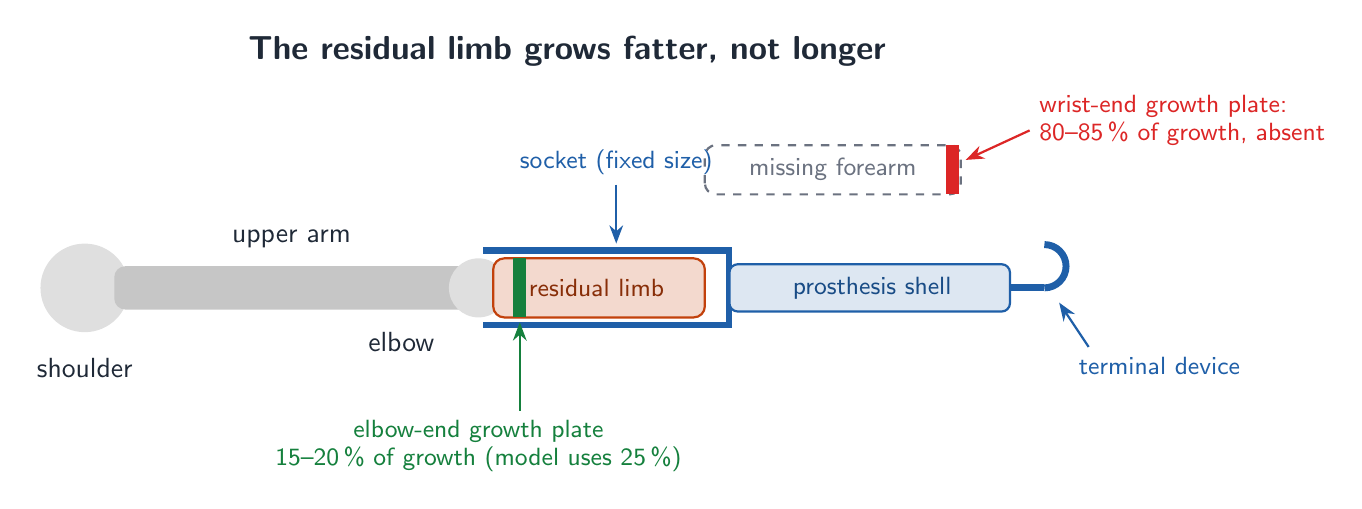
\begin{tikzpicture}[scale=1.25]
\fill[gray!25] (0,0) circle (0.45); \node[below=6pt] at (0,-0.45) {shoulder};
\fill[gray!45,rounded corners=4pt] (0.3,-0.22) rectangle (4,0.22); \node at (2.1,0.5) {upper arm};
\fill[gray!25] (4,0) circle (0.3); \node[left] at (3.65,-0.55) {elbow};
\fill[limb!20,draw=limb,thick,rounded corners=4pt] (4.15,-0.3) rectangle (6.3,0.3);
\node[limb!70!black] at (5.2,0) {\small residual limb};
\fill[good] (4.35,-0.3) rectangle (4.48,0.3);
\draw[pro,line width=2.2pt] (4.05,0.38)--(6.55,0.38)--(6.55,-0.38)--(4.05,-0.38);
\fill[pro!15,draw=pro,thick,rounded corners=3pt] (6.55,-0.24) rectangle (9.4,0.24);
\node[pro!80!black] at (8,0) {\small prosthesis shell};
\draw[pro,line width=2.5pt] (9.4,0)--(9.75,0); \draw[pro,line width=2.5pt] (9.75,0) arc (-90:90:0.22);
\draw[dashed,quiet,thick,rounded corners=4pt] (6.3,0.95) rectangle (8.9,1.45);
\node[quiet] at (7.6,1.2) {\small missing forearm};
\fill[hot] (8.75,0.95) rectangle (8.88,1.45);
\draw[->,thick,good] (4.42,-1.25)--(4.42,-0.35); \node[good,align=center,below] at (4.0,-1.25) {\small elbow-end growth plate\\[-2pt]\small 15--20\,\% of growth (model uses 25\,\%)};
\draw[->,thick,hot] (9.6,1.6)--(8.95,1.3); \node[hot,align=left,right] at (9.6,1.7) {\small wrist-end growth plate:\\[-2pt]\small 80--85\,\% of growth, absent};
\draw[->,thick,pro] (5.4,1.05)--(5.4,0.45); \node[pro,above] at (5.4,1.05) {\small socket (fixed size)};
\draw[->,thick,pro] (10.2,-0.6)--(9.9,-0.15); \node[pro,below right] at (10.0,-0.6) {\small terminal device};
\node[font=\large\bfseries] at (4.9,2.4) {The residual limb grows fatter, not longer};
\end{tikzpicture}
\end{document}
